

\subsection{signal details}
\label{sec:signaldetail}

The Signal class should be able to support multiple dimensions for arguments (time, channel, space, ...) and values (TX power, attenuation, bitrate). That means both sides of our signal function have to be extendable.

The following section explains how we achieve this.

\subsubsection{multiple dimensions for values}

Generally spoken a function can be implemented as a map from ``Argument`` to
''Value``. With inheritance we could basically use everything as a Value.
If we assume that every Value of our Signals is in $\mathbb{R}^n$ we could
implement it as a vector of doubles of size \textit{n}.

\subsubsection{multiple dimensions for arguments}

While we could use basically everything as Value the Argument has to be
distinguishable. Further a simple map with an Argument class as key would be
hard to iterate reasonable and fast.

So instead of using one map from Argument to Value we realize multiple
dimensions by using sub signals (see figure \ref{fig:signalscheme}). We add a
dimension of arguments by implementing a map from the argument value to another
sub-signal. This structure has three advantages:

\begin{enumerate}
\item The Signal dimensions are easy to extend.
\item It provides a deterministic way to iterate over it.
\item And if every sub signal knows its dimension we can still use an Argument class (which would be, same as the Value, an extendable vector of doubles) for direct access to a specific Value of the Signal.
\end{enumerate}


\begin{figure}[H]
 \centering
 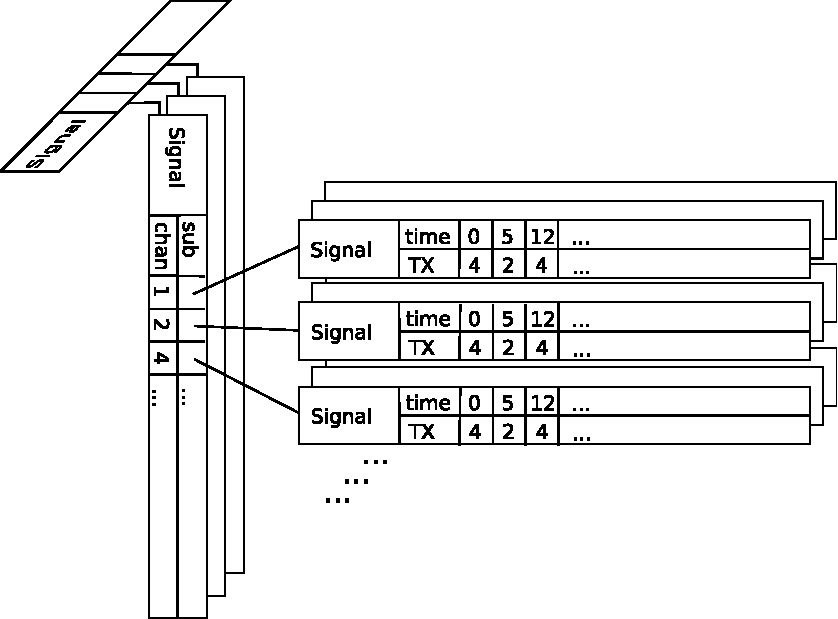
\includegraphics[width = 0.8\textwidth]{SignalDetail/signal_scheme.pdf}
 \caption{multi dimensional signals}
 \label{fig:signalscheme}
\end{figure}

\subsubsection{creating and identifying Signals}

Three things have to be considered:

\begin{enumerate}
\item We have three classes now (Signal, Argument and Value) which depends all on the type (meaning the dimensions) of the Signal. So we have to make sure to create the appropriate Arguments and Values for a Signal.
\item A receiving physical layer could receive different types of Signals during runtime, so we need a way to identify the type of a Signal.
\item The Signal types have to be globally known by each Physical Layer in the simulation.
\end{enumerate}

We solve the first two problems by introducing a SignalPrototype class. If we want to create a new Signal type we create a new SignalPrototype with the parameters for the Signal type (which would be the dimensions). The SignalPrototype then is able to create the appropriate Signals, Arguments and Values. It is also used as Identifier for the Signal type.

The last problem is solved by a simulation wide known SignalDatabase which maps 
a Signal type name ("MIMO signal" for example) to the associated Prototype.
Every new SignalPrototype has to be registered by a unique name with the
SignalDatabase. 

\subsubsection{detailed class diagram of Signal}

The above decisions lead to the following class diagram:

\begin{figure}[H]
 \centering
 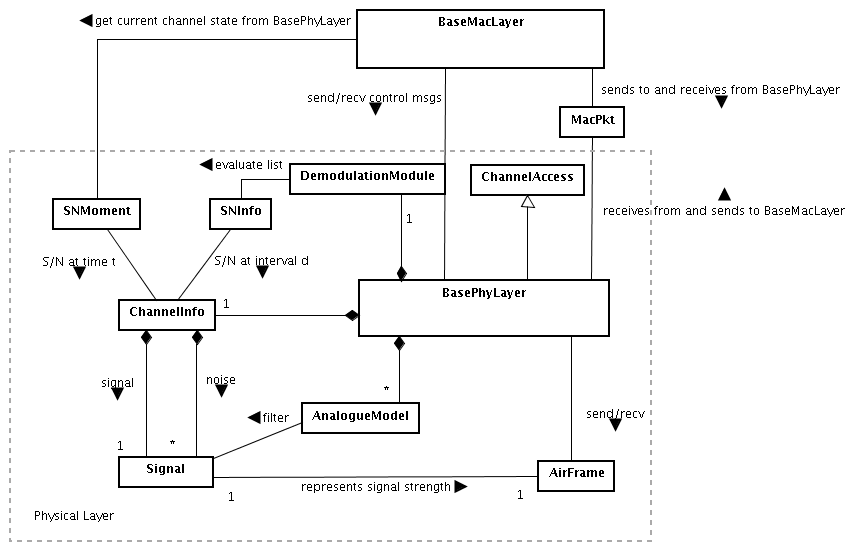
\includegraphics[width = \textwidth]{SignalDetail/class_diagram.png}
 \caption{detailed class diagram}
 \label{fig: signal classgraph}
\end{figure}

\newpage
\subsubsection{creation of new signal types}

To assure that every new SignalPrototype is registered with the database we
don't provide a public constructor for the SignalPrototype. If a physical layer
wants to create a new prototype it has to ask the database if a prototype with
the same name is already registered. If not it can ask the database to create a
new one with the given name.\\

We assume that every Signal has at least time as argument dimension and TX 
power and attenuation as value dimensions. So these dimensions are already
included in every new prototype.

Additional dimensions have to be registered by name with the prototype. The 
registration methods returns a unique sequential number for the registered
dimension. This number is used later as a fast way to access the values of the
dimension.

If every dimension is registered at the prototype one can create proper new 
Signals, Arguments and Values with this SignalPrototype.\\

\emph{Note: The first time the SignalPrototype is used to create a Signal, 
Argument or Value it is internally locked and no other dimensions can be
registered.}\\

The "isPrototypeFor()" method can be used to check if a Signal was created by 
this Prototype.

\begin{figure}[H]
 \centering
 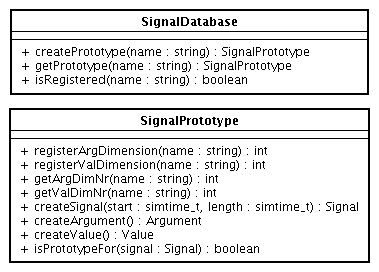
\includegraphics[width =  0.8\textwidth]{SignalDetail/database_members.png}
 \caption{interface of Database and Prototype}
 \label{fig: Database members}
\end{figure}
\newpage
\subsubsection{accessing the Signal}

The following class diagram shows the methods which the Signal provides
\textbf{additionally} to those listed in figure \ref{fig:memberAirFrame}.

\begin{figure}[H]
 \centering
 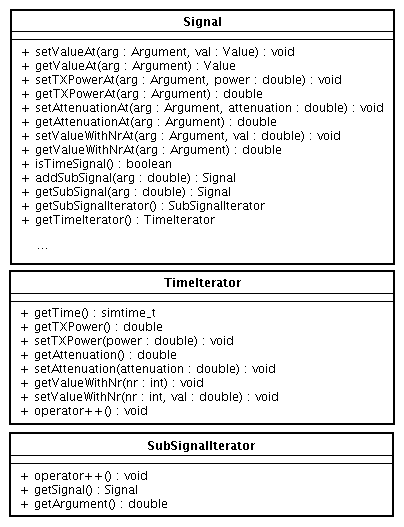
\includegraphics[width =  0.8\textwidth]{SignalDetail/signal_members.png}
 \caption{signal interface details}
 \label{fig: detailed signal members}
\end{figure}

The TimeIterator still iterates over every time stamp of the Signal, independent
from the dimension of the Signal. This way simple filters can be applied without
knowledge of the exact type of the Signal.\\

The easiest way to access a specific value of the Signal, is to create an 
instance of the apropriate Argument (and Value, if you want to change it),
initialize its dimensions with the wanted values and then use the "getValueAt()"
and "setValueAt()" methods. Here one has to know that an entry for the given
Argument actually exists, otherwise the Signal would have to interpolate the
Value.\\

The SubSignalIterator can be used to iterate recursively over every pair of 
value and its associated sub signal of the dimension this Signal represents. The
deepest SubSignal will always be the time dimension which can be checked by
"isTimeSignal()".

\begin{figure}[H]
 \centering
 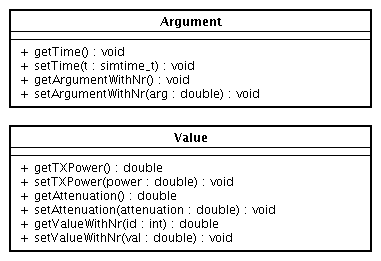
\includegraphics[width =  0.8\textwidth]{SignalDetail/argval_members.png}
 \caption{interface for Argument and Value}
 \label{fig: arg and val members}
\end{figure}

The SignalPrototype associates every argument dimension name with a unique 
sequential number. The same holds for the value dimensions. These numbers can be
used to access the values in Argument or Value with the 
"get*WithNr()" methods.

Because every Argument has a time dimension and every Value a TX power and an 
attenuation, the classes provide short cuts to these values.
